Svi zadaci ostvareni su u okviru učenja pretraživanja koji je implementiran u
sustavu za strojno učenje zvanom Vowpal Wabbit. U dodacima
\ref{appendix:postagging}, \ref{appendix:msdattr}, \ref{appendix:msdlayered}
prikazana je jednostavnost implementacije za zadatke označavanja vrste riječi.
Korišten je programski jezik \textsc{C++}. Moguće je sve zadatke izvesti u
jeziku \textsc{Python}, ali ušteda u čitljivosti smanjuje vremensku
učinkovitost. Uzevši u obzir da je okvir učenja pretraživanja poprilično
modularan tijekom implementacije greške su uglavnom bile prisutne u krivoj
obradi podataka i odabiru hiperparametara. \textit{Hashing trick} dozvoljava
običan tekstualni format za svaku značajku stoga je ulazna datoteka vrlo
jednostavna (dodatak \ref{appendix:data}).

\citet{daume14lts} opisuju efikasnu implementaciju okvira učenja pretraživanja.
Na slici \ref{fig:ltsperf} prikazana je vremenska učinkovitost sustava na
zadatku označavanja vrste riječi i imenovanim entitetima -- broj označenih
tokena po sekundi. Učinkovitost je prisutna i kod ostvarenih rješenja za
probleme obrađene u okviru ovog rada.

\begin{figure}
  \centering
  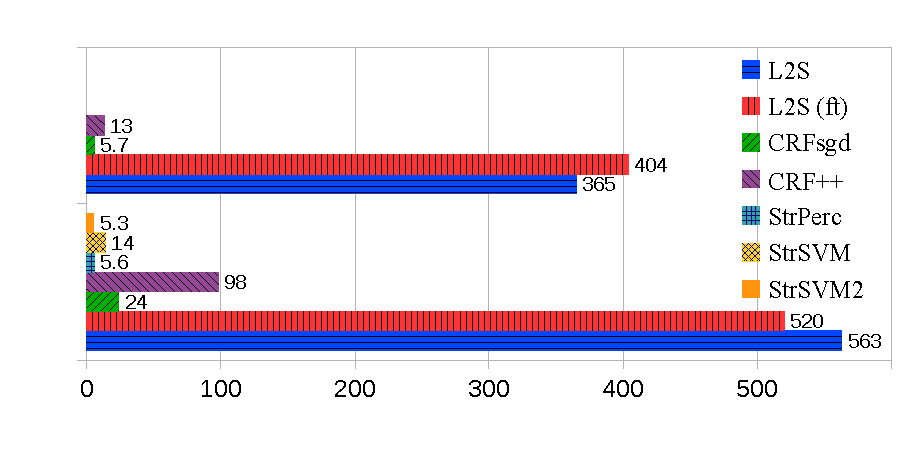
\includegraphics[scale=0.9]{tokenposec.pdf}
  \caption[Usporedba brzine označavanja metoda strukturnog
  predviđanja.]{Usporedba brzine označavanja metoda strukturnog predviđanja.
  Prikazani brojevi su u tisućama po sekundi. Slika se u izvornom obliku nalazi
  u \citep{ltsicmltutorial}.}
  \label{fig:ltsperf}
\end{figure}
